% !TEX root = ../../main.tex

\section{A case study of high throughput processing on a large dataset}

\subsection{The NIST ISOD dataset}

The NIST/ARPA-E database of adsorbent materials (ISODB) is a comprehensive
set of adsorption isotherms which have been systematically
collected from peer-reviewed literature. The data includes 
measurements on a wide range of materials, from carbon, zeolite,
and silica to MOFs and other such PCPs. This resource is a useful
tool for reference purposes, as it contains isotherms on many reported
porous materials. Furthermore, due to the availability of an 
application programming interface (API), isotherm data can be easily
accessed. As such, this database is a great 
source of data for the kind of large-scale processing which pyGAPS
is designed for.

The entire dataset in the NIST adsorption database was downloaded using the
publicly available API. This yielded \(\approx \! 26000\) isotherms.
In order to narrow down the dataset and ensure comparable starting values
some sorting was performed.

\begin{itemize}
    \item Isotherms which could not be converted to \si{\milli\mol\per\gram}
    were discarded outright. This includes data reported in a 
    on a volume basis of material (as the material density is 
    unknown), simulation data which is reported in units such 
    as molecules per unit cage and fractional coverage isotherms.
    \item No isotherms with less than 6 measurement points were 
    considered, as sufficient datapoints are needed for characterisation.
    \item Isotherms were then converted into \si{\milli\mol\per\gram},
    to ensure a consistent unit set.
    \item Possible outliers were removed from the data by selecting 
    only isotherms recorded under \SI{100}{\bar}, with maximum capacities
    under \SI{100}{\milli\mol} and with a temperature of under 
    \SI{443}{\kelvin}. Any such isotherms are likely errors in the 
    data collection process and have little to no physical meaning.
\end{itemize}

The process of data collation reduced the number of isotherms
to \(\approx \! 15800\). A distribution of the isotherms as a 
function of adsorbate and temperature can be found 
in \autoref{pyg:fgr:nist-dataset}.
We can see that most isotherms are recorded at either 
\SI{77}{\kelvin}, \SI{273}{\kelvin} or \SI{298}{\kelvin} as 
these are temperatures are readily available through immersion
in liquid nitrogen, water-ice mixture, or a thermally controlled
water bath.

\begin{figure}[htb]
    \centering

    \begin{subfigure}{0.5\linewidth}
        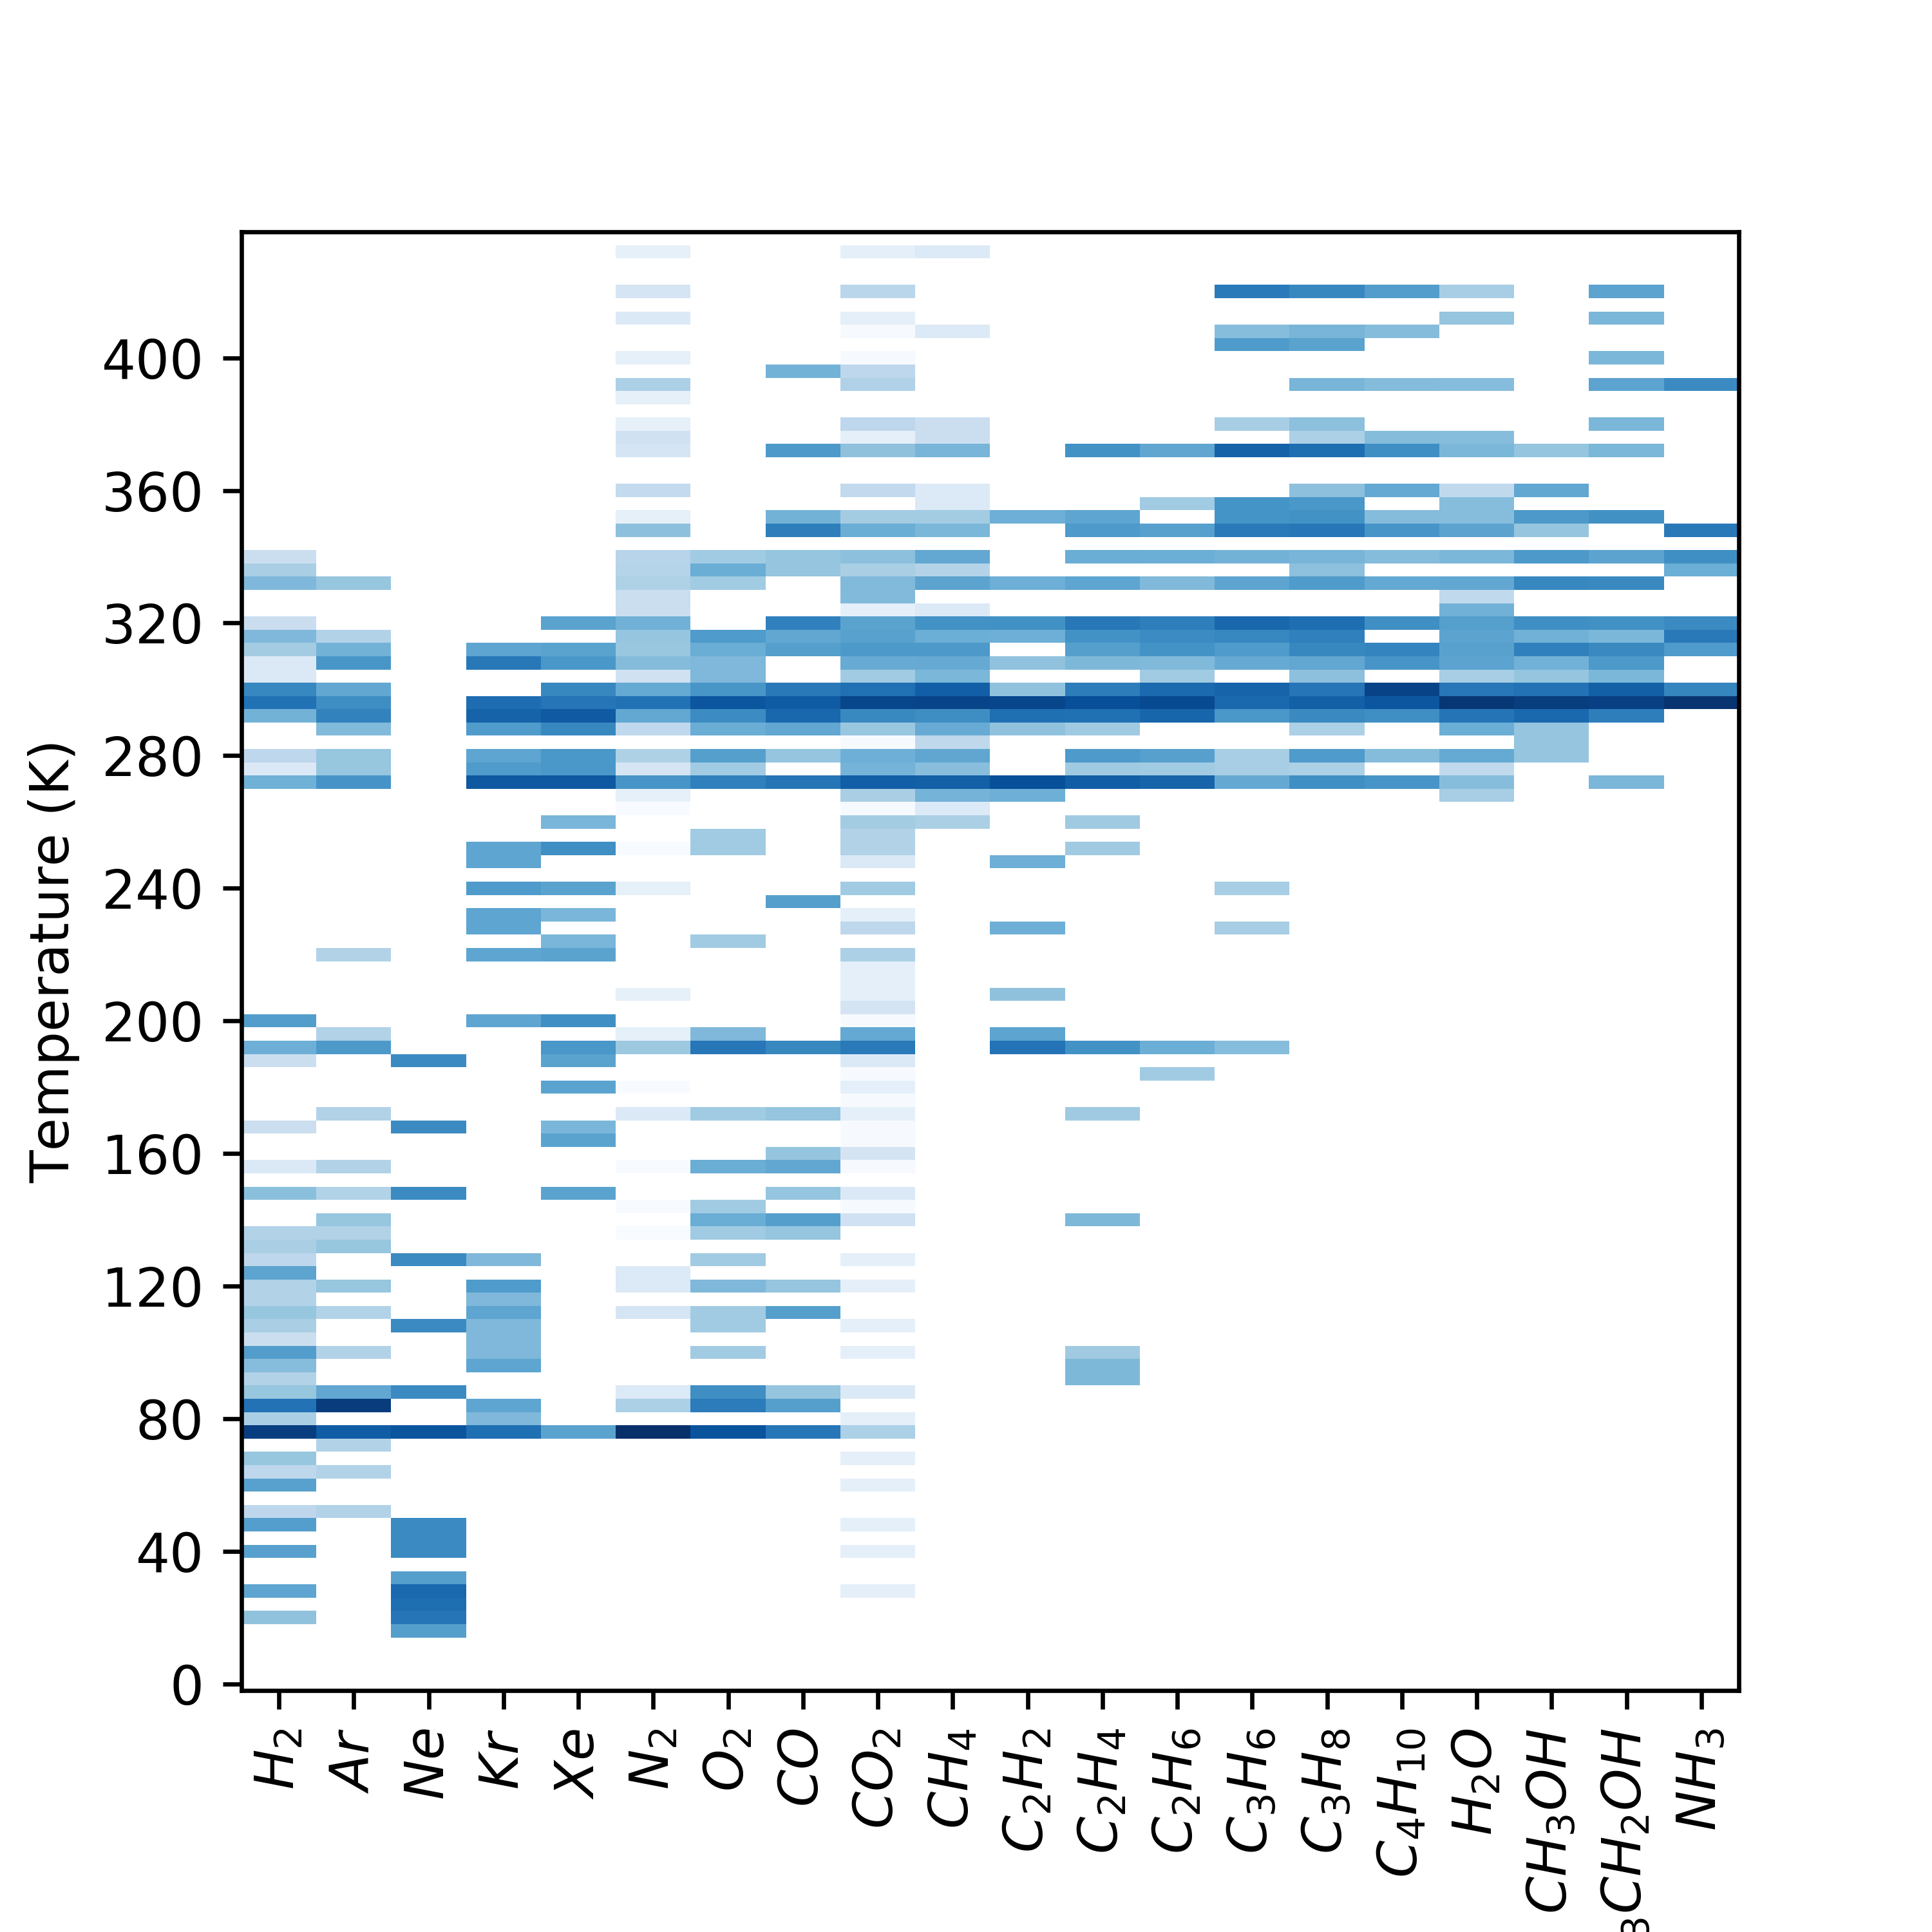
\includegraphics[width=\linewidth]{nist/nist-dataset}%
        \caption{}%
        \label{pyg:fgr:nist-dataset}
    \end{subfigure}%
    \begin{subfigure}{0.4\linewidth}
        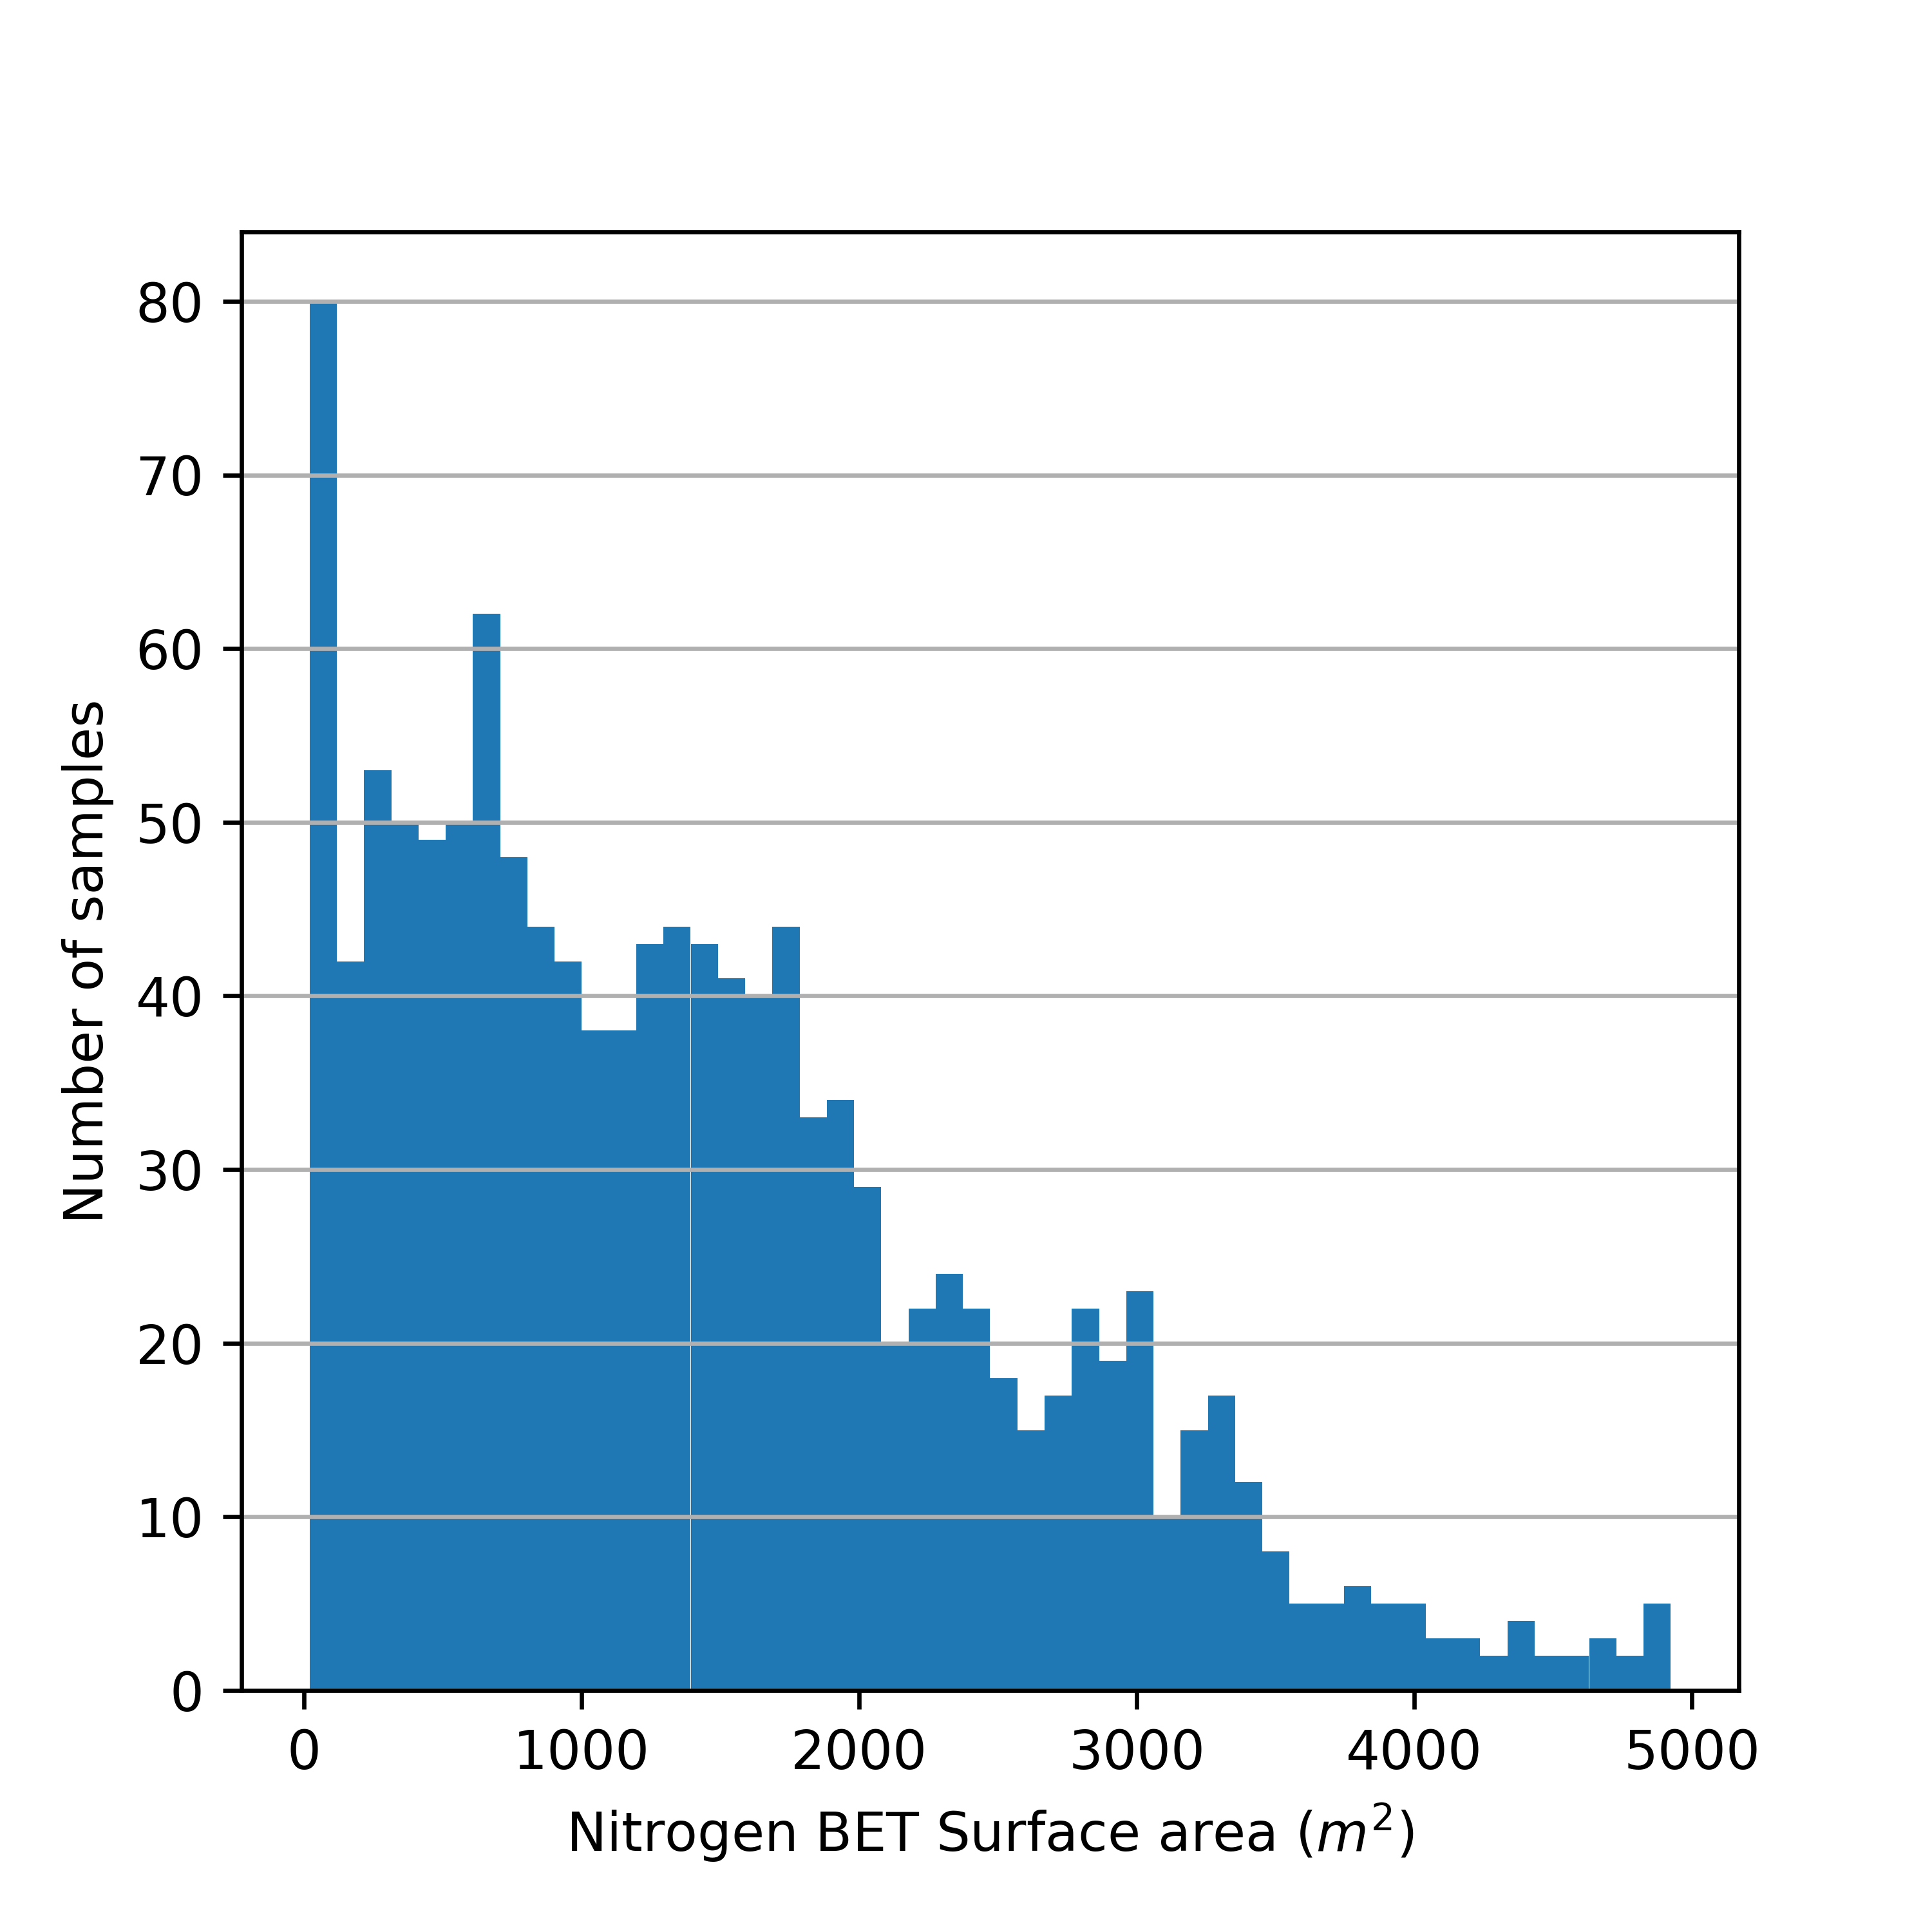
\includegraphics[width=\linewidth]{nist/nist-bet-area}%
        \caption{}%
        \label{pyg:fgr:nist-dataset-area}
    \end{subfigure}%

    \caption{A graphical description of the NIST ISODB dataset.
    (a) The selected 15800 isotherms presented per adsorbate used
    and temperature at which the measurement took place.
    (b) Calculated BET surface area with nitrogen at \SI{77}{\kelvin}
    for all available isotherms. }%
    \label{pyg:fgr:nist-set}
\end{figure}

To apply the high throughput data processing with pyGAPS,
only isotherms recorded with nitrogen at \SI{77}{\kelvin}
were selected. These make up \(\approx \! 3500\) datapoints,
recorded on more than 2200 materials. The BET surface area 
was then computed for each isotherm, with a distribution
as seen in \autoref{pyg:fgr:nist-dataset-area}.
Unfortunately, as many isotherms do not have enough points
in the low pressure region, computing a well-defined
BET surface area is impossible. In total, only around a
third of the isotherms had enough data for this purpose.

Quite a few materials are seen to be essentially non-porous
with a more than 80 isotherms with a BET area of less 
than \SI{100}{\metre^2}.

\subsection{A comparison between surface area determination methods}

It is also useful to observe the differences between the 
Langmuir-calculated and the BET-calculated surface areas.
If the Langmuir area is calculated with implicit parameters,
by taking the entire available isotherm for the fitting
routine, the correlation between the surface areas
calculated through the two methods is presented in 
\autoref{pyg:fgr:nist-bet-langmuir}. The Langmuir surface 
area is generally higher than the BET surface area for the 
same isotherm. This is a consequence of the 

If the partial pressure range is narrowed, by only using 
points up to 0.2 \(p/p_0\), the correlation improves 
dramatically, with near-overlap when the area is below 
\SI{200}{\metre^2}. The better ,

It should also be noted that the, as shown by 
\citeauthor{waltonApplicabilityBETMethod2007}
~\cite{waltonApplicabilityBETMethod2007} when attempting to
compare nitrogen surface areas with BET-calculated 
surface areas for MOFs and microporous materials.

\begin{figure}[htb]
    \centering

    \begin{subfigure}{0.42\linewidth}
        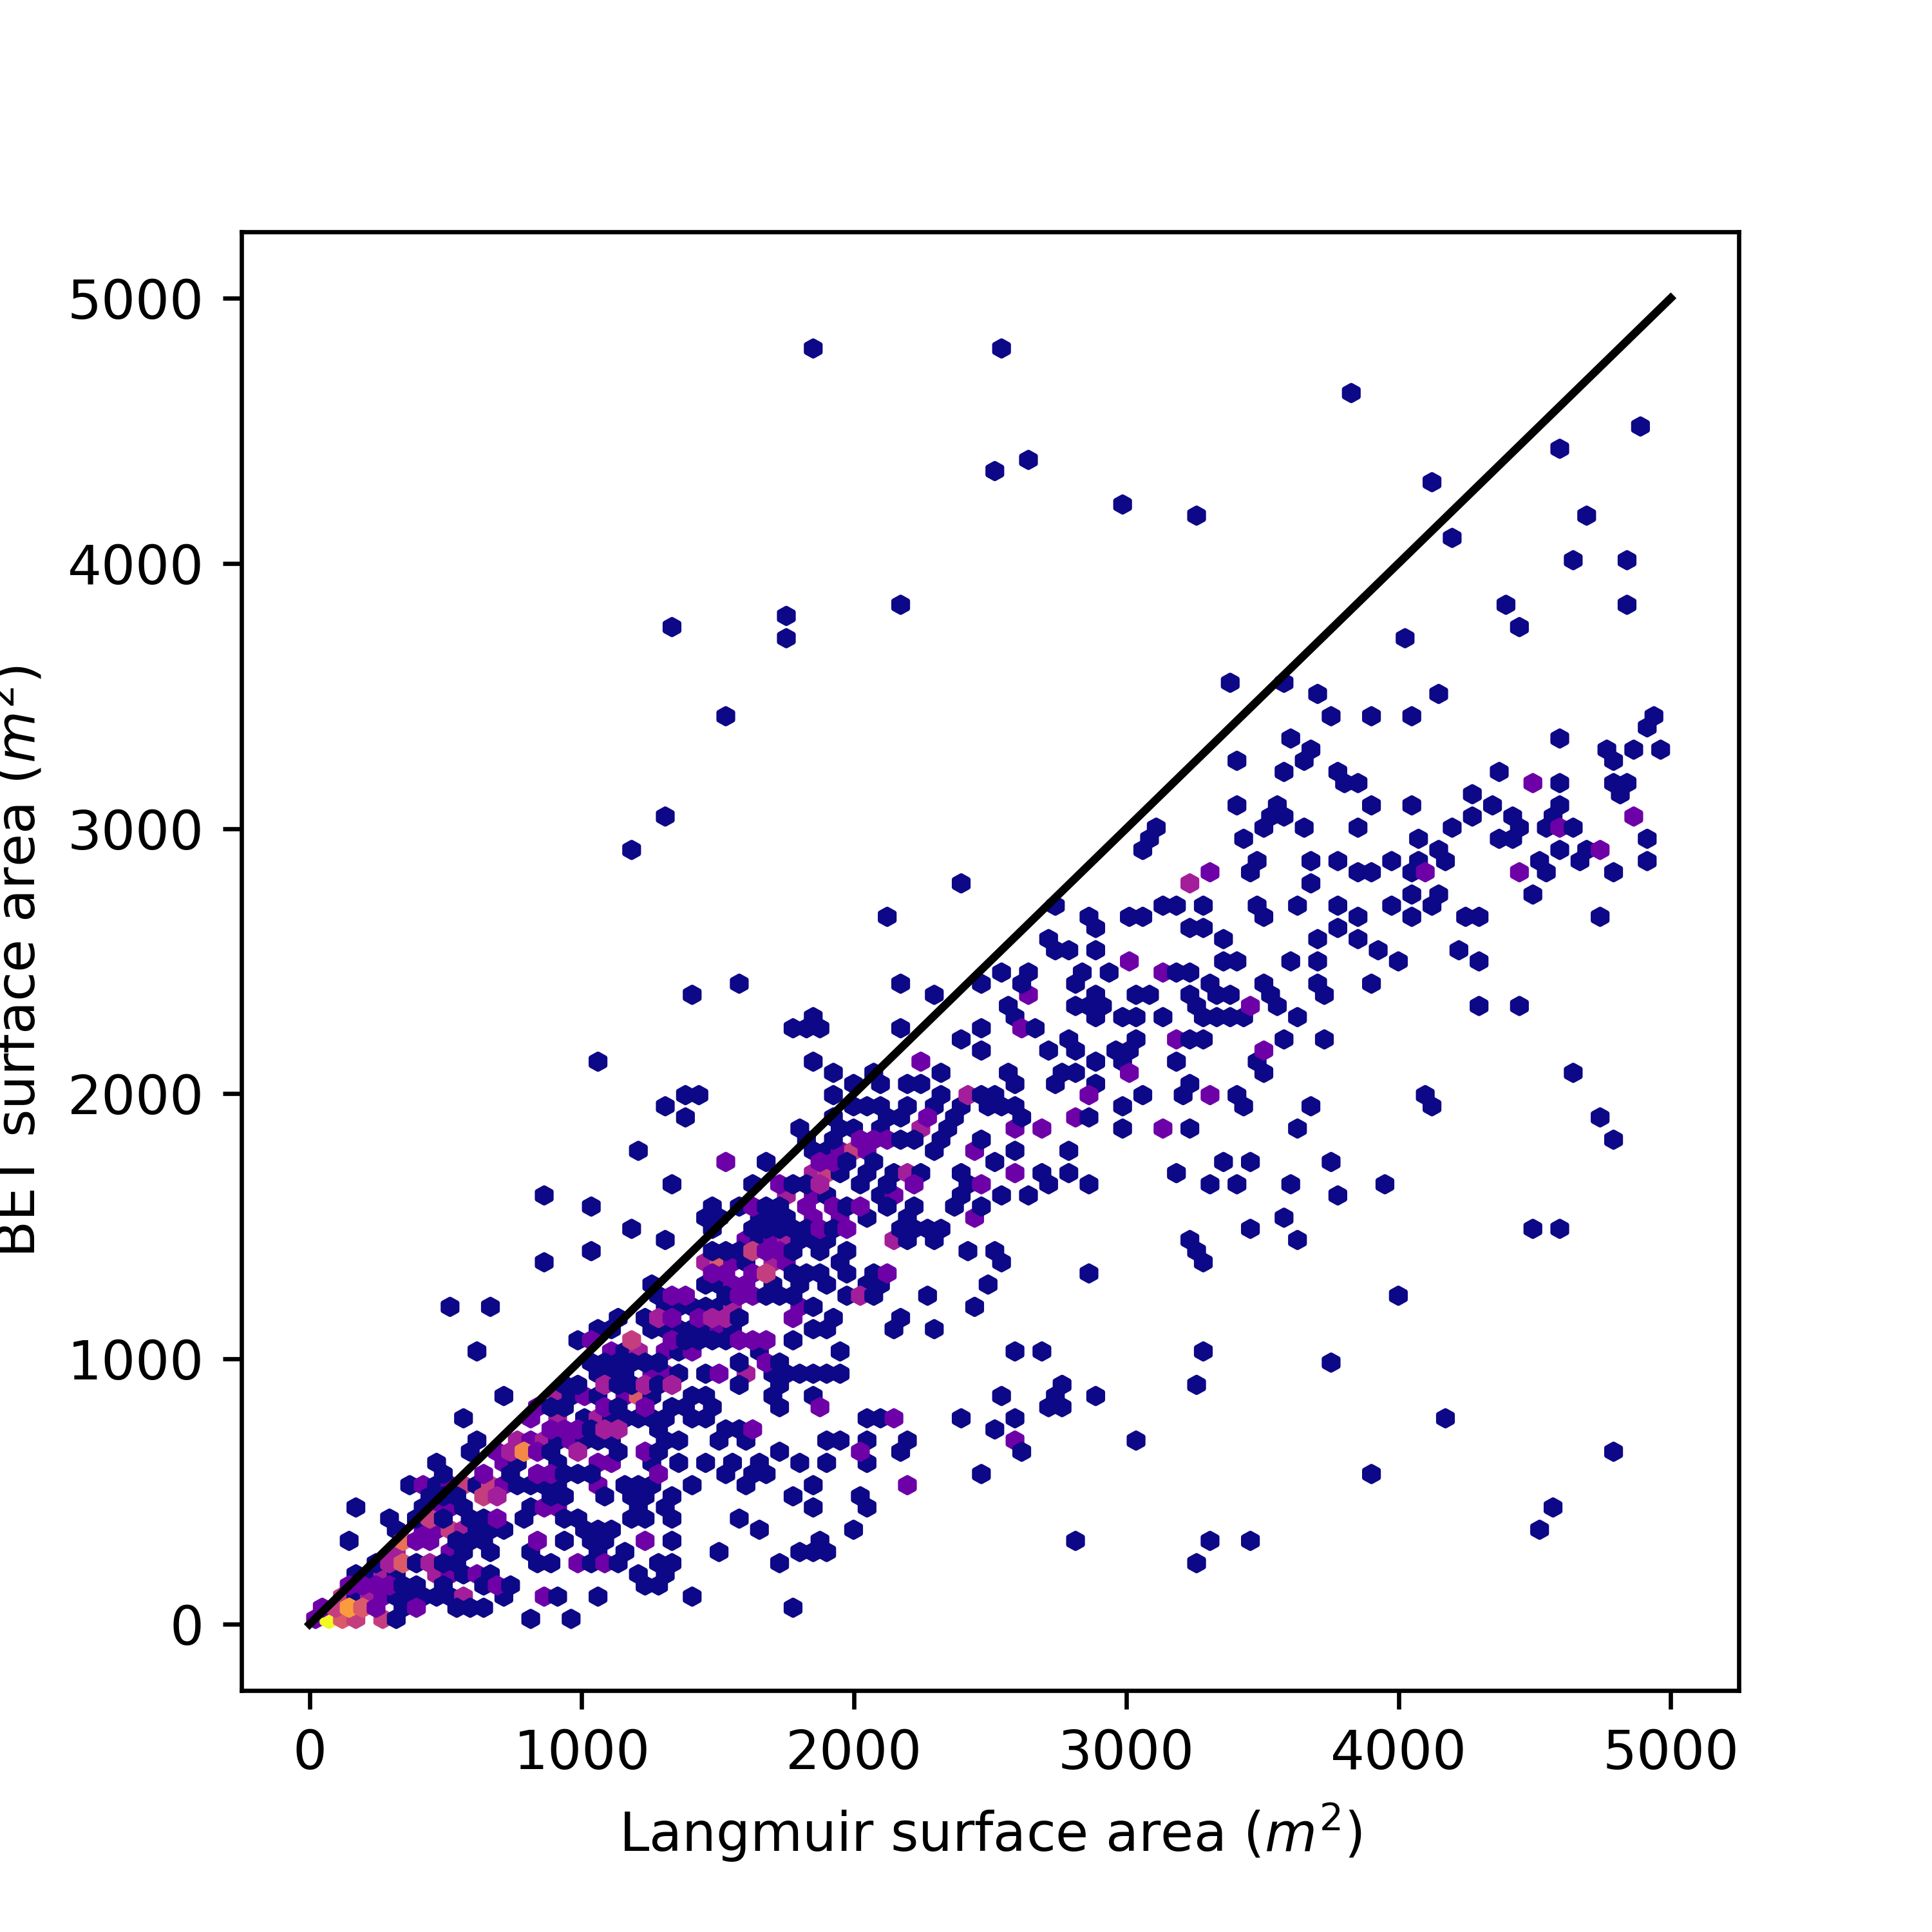
\includegraphics[width=\linewidth]{nist/nist-bet-langmuir}
        \caption{Full range}%
        \label{pyg:fgr:nist-bet-langmuir}
    \end{subfigure}%
    \begin{subfigure}{0.5\linewidth}
        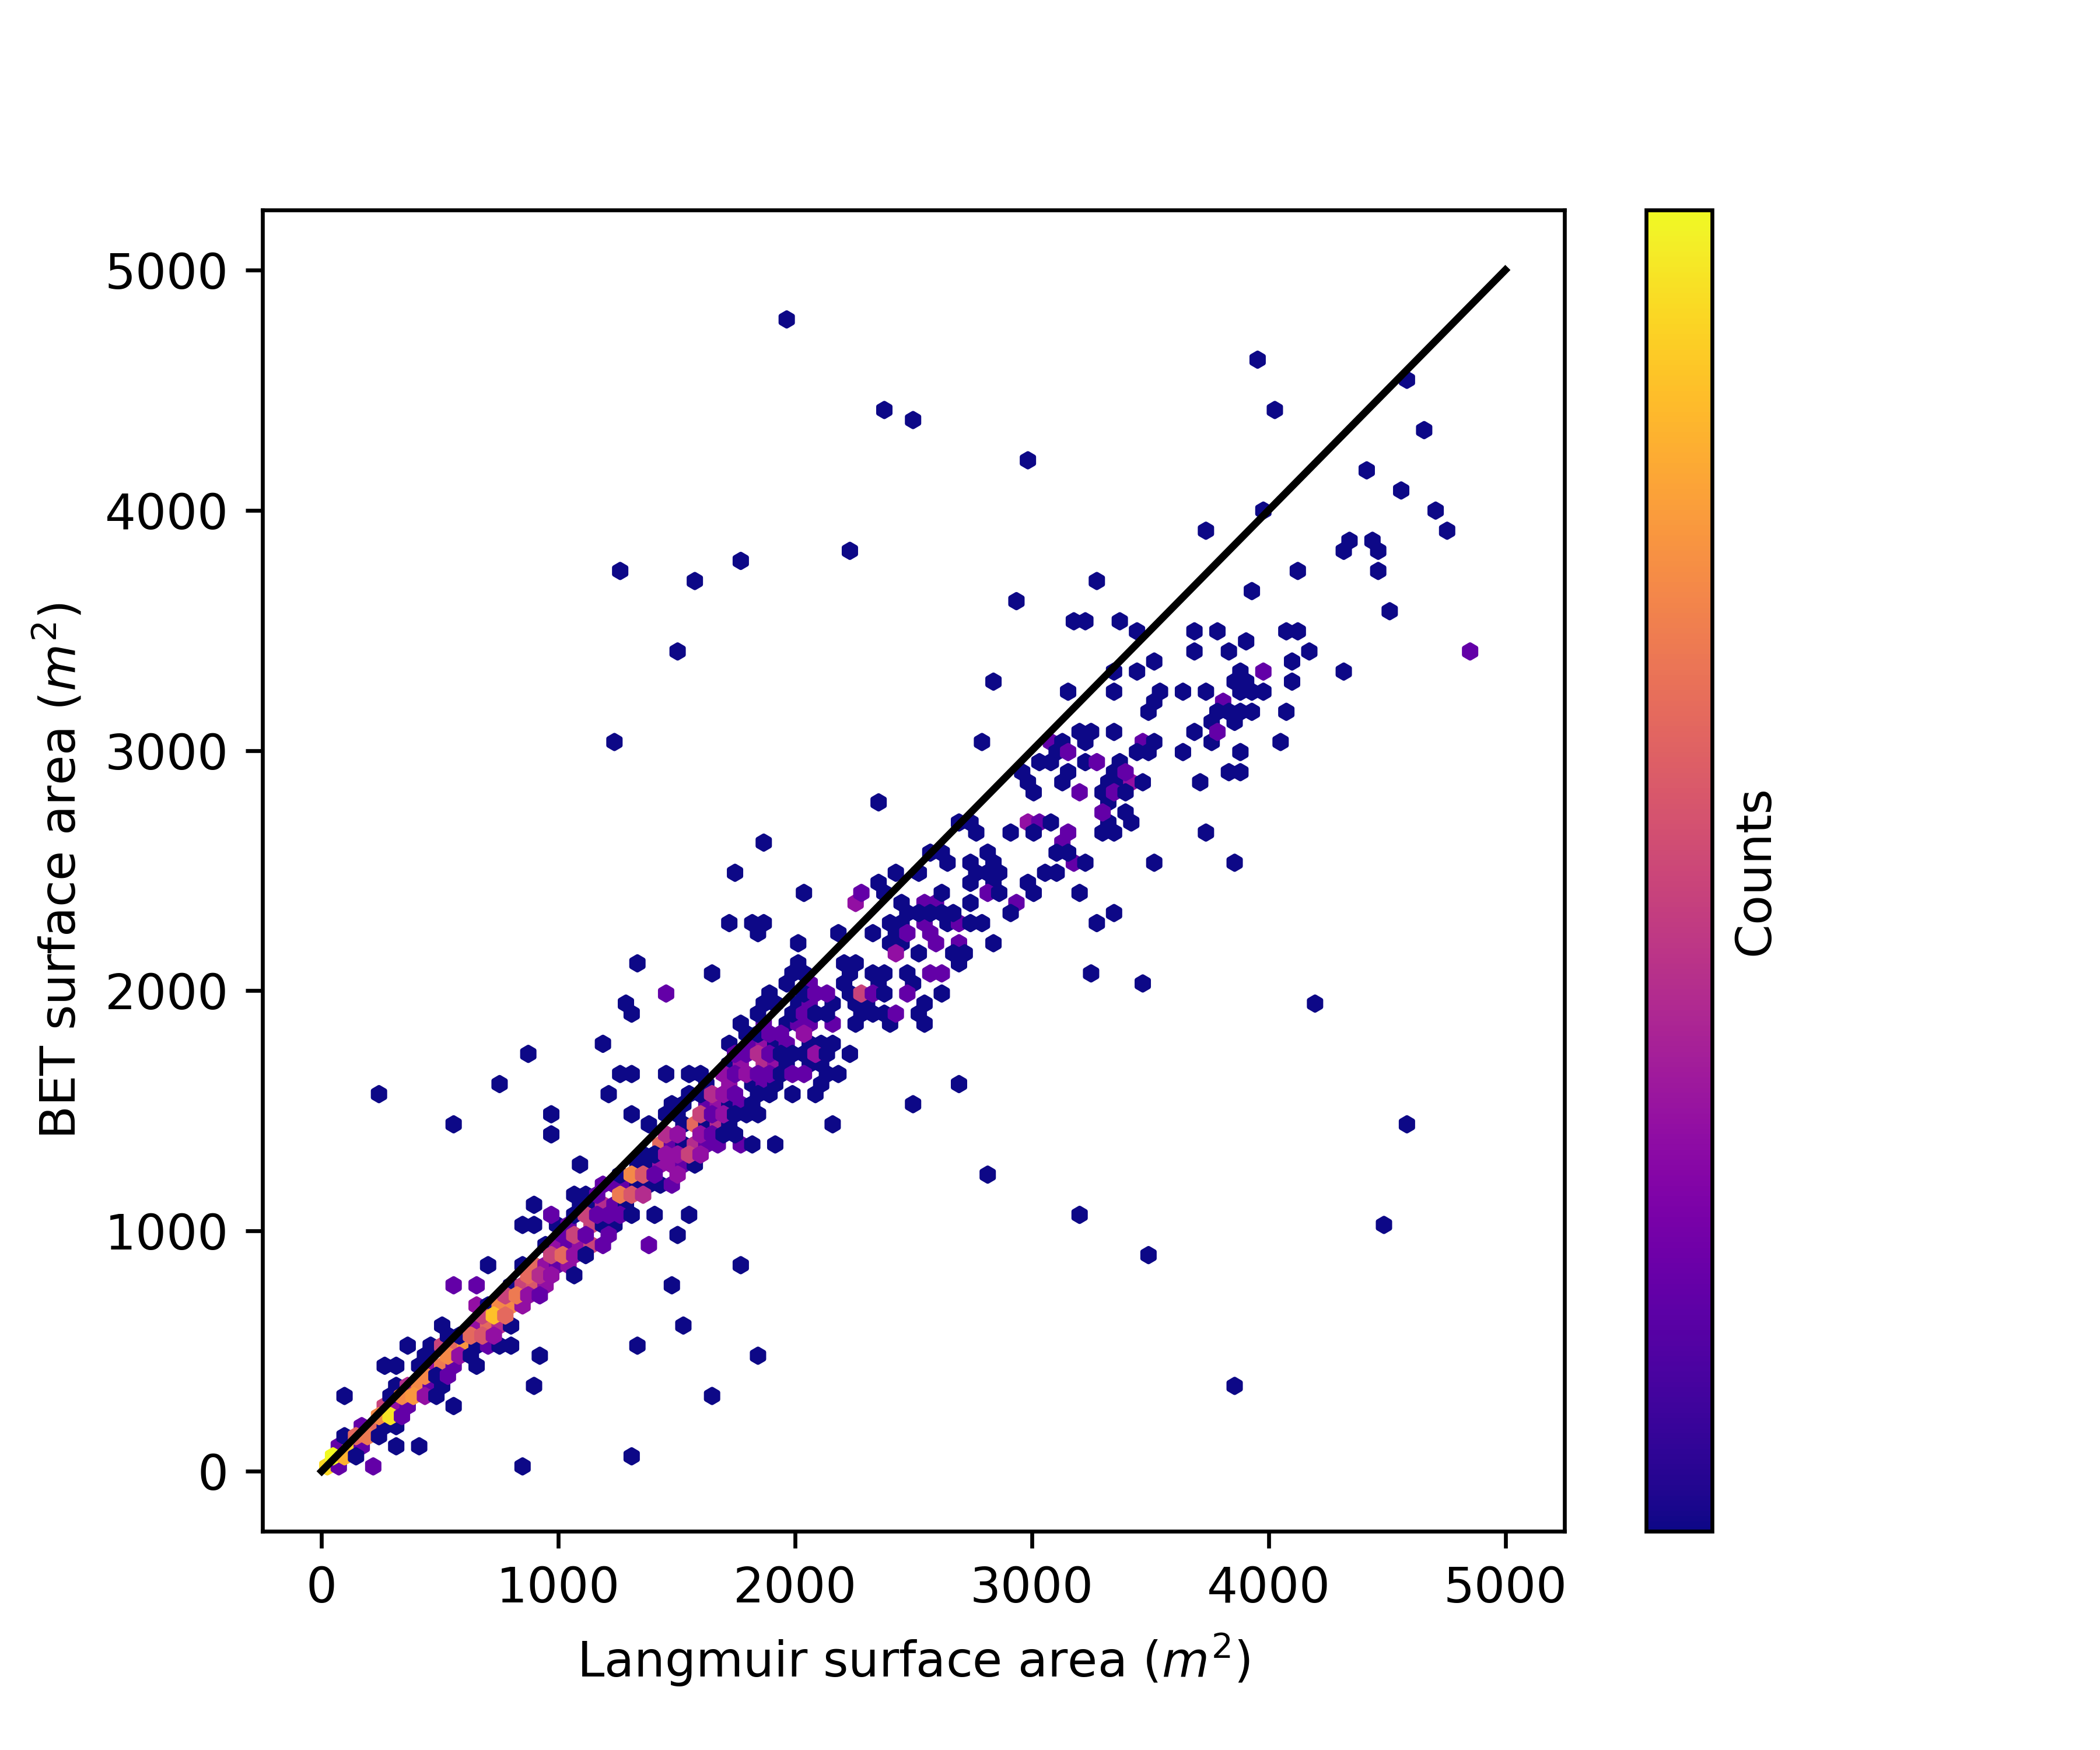
\includegraphics[width=\linewidth]{nist/nist-bet-langmuir-2}
        \caption{0--0.2 \(p/p_0\) range}%
        \label{pyg:fgr:nist-bet-langmuir-adj}
    \end{subfigure}%

    \caption{Correlation between Langmuir-calculated and 
    BET-calculated surface areas. The black line is a guide
    for the eye at \(S_{langmuir} = S_{BET}\).}%
    \label{pyg:fgr:nist-area-cmp}
\end{figure}

To go one step further into uncovering trends for 

\subsection{Observed reliability of results}

Recently, Sholl and co-workers~\cite{parkHowReproducibleAre2017}
have published a report putting into question the reproducibility
or adsorption isotherms, using \ce{CO2} adsorption data from the 
NIST ISODB. Their findings highlight a large variability inherent
to reported isotherms as on average \textit{``one in five \ce{CO2} 
isotherms [\ldots] cannot be used to provide information that 
is qualitatively reliable about the properties of the material''}.
In this paper no reasons behind the origin of such large
variations in reproducibility are explored. Similar concerns have been
raised for \ce{H2}~\cite{broomIrreproducibilityHydrogenStorage2016}
and \ce{CO2}~\cite{espinalMeasurementStandardsData2013} measurements.

The underlying cause for the poor reproducibility of adsorption
isotherms, particularly those measured on metal organic frameworks
is not easy to pinpoint. A large contribution to this divergence
is likely accounted for through the variation introduced by the
sample preparation method and adsorption apparatus.
For example, a recent NIST interlaboratory study in which \ce{CO2} 
isotherms were recorded on a reference 
material~\cite{nguyenReferenceHighpressureCO22018}, had six 
out of thirteen initial datasets outside the uncertainty range.
Errors were determined to arise from sample mass measurement,
insufficient activation conditions or improper choice of an 
equation of state. Other method-specific sources of error exist,
such as the lack of a buoyancy correction when using a 
gravimetric system or a void volume correction when using 
a volumetric system, both of which can made if an accurate
determination of sample skeletal density is performed. Finally,
small differences in thermal gradients, pressure transducer
readings, and even the altitude at which the measurement takes place
(if a phase change bath is used to control temperature)
can also impact the final isotherm.

Such variation is likely minimised when using state-of-the-art 
adsorption equipment, which eliminates many of the concerns
associated with adsorption methodology. \textit{In situ}
activation, internal consistency checks for pressure transducers,
automatic measurement of skeletal density and associated 
corrections, reference cells for saturation pressure determination
and many other sanity checks are implemented in these machines.

However, it is often the case that the most important factor
in the repeatability MOF and porous material adsorption isotherms 
is not the measurement procedure, but rather the material itself.
